\documentclass{beamer}
\usepackage[utf8]{inputenc}
\usepackage{tikz}
\usepackage{svg}
\usepackage{drawstack}
\usepackage[dvipsnames,svgnames,table,hyperref]{xcolor}
\usetikzlibrary{calc, arrows}
\usetikzlibrary{shapes.multipart} %for the stack
\usepackage{listings} 
\usepackage{mathtools}
\usepackage{amsthm}
\usepackage{kbordermatrix} %for the representations
\pgfdeclarelayer{background} %tiks animation stuff
\pgfsetlayers{background,main}
\usetheme{metropolis}           % Use metropolis theme
\title{Graph Theory}
\date{\today}
\author{Dadams, TEC, Nick, Tom}
\institute{Graph This!}
\begin{document}


\section{Graph Algorithms: \\ DO U KNOW DE \sout{WAY} PATH}
\begin{frame}{Searching}
    The first algorithms we are going to cover enumerate or search for all possible paths in a graph, not just one:
    \begin{itemize}
        \item Breath First Search
        \item Depth First Search
    \end{itemize}
\end{frame}
\tikzstyle{vertex}=[circle,draw=blue!40!white, black=blue, fill=white!10!white, minimum size=0.75cm]
\tikzstyle{selected vertex} = [vertex, fill=red!24]
\tikzstyle{edge} = [draw,thick,-]
\tikzstyle{weight} = [font=\small]
\tikzstyle{selected edge} = [draw,line width=5pt,-,red!50]
\tikzstyle{ignored edge} = [draw,line width=5pt,-,black!20]

\begin{frame}{Breath First Search}
\centering
\begin{tikzpicture}[scale=2.5, auto,swap]
    % First we draw the vertices
    \foreach \pos/\name in {
                                {(1.5,2.5)/0},
                                {(0.25,1.75)/1}, {(2.75,1.75)/2},
                                {(-0.25,1)/3}, {(0.75,1)/4}, {(2.25,1)/5}, {(3.25,1)/6},
                                {(-0.25,0.25)/7}, {(0.5,0.25)/8}, {(1,0.25)/9}, {(1.75,0.25)/10}, {(2.25,0.25)/11}, {(2.75,0.25)/12}}
        \node[vertex] (\name) at \pos {$\name$};
    % Connect vertices with edges and draw weights
    \foreach \source/ \dest /\weight in {0/1/, 0/2/,1/3/,1/4/,
                                         3/7/, 4/8/,4/9/,
                                         0/2/,2/5/,
                                         2/6/,5/10/,5/11/,5/12/}
        \path[edge] (\source) -- node[weight] {$\weight$} (\dest);
\end{tikzpicture}
\end{frame}

\begin{frame}{BFS}

\begin{figure}
\begin{tikzpicture}[scale=2.5, auto,swap]
    % First we draw the vertices
    \foreach \pos/\name in {
                                {(1.5,2.5)/0},
                                {(0.25,1.75)/1}, {(2.75,1.75)/2},
                                {(-0.25,1)/3}, {(0.75,1)/4}, {(2.25,1)/5}, {(3.25,1)/6},
                                {(-0.25,0.25)/7}, {(0.5,0.25)/8}, {(1,0.25)/9}, {(1.75,0.25)/10}, {(2.25,0.25)/11}, {(2.75,0.25)/12}}
        \node[vertex] (\name) at \pos {$\name$};
    % Connect vertices with edges and draw weights
    \foreach \source/ \dest /\weight in {0/1/, 0/2/,1/3/,1/4/,
                                         3/7/, 4/8/,4/9/,
                                         0/2/,2/5/,
                                         2/6/,5/10/,5/11/,5/12/}
        \path[edge] (\source) -- node[weight] {$\weight$} (\dest);
    % Start animating the vertex and edge selection. 
    \foreach \vertex / \fr in {0/0,1/1,2/1,3/2,4/2,5/3,6/3,7/4,8/5,9/5,10/6,11/6,12/6}
        \path<\fr-> node[selected vertex] at (\vertex) {$\vertex$};
    % For convenience we use a background layer to highlight edges
    % This way we don't have to worry about the highlighting covering
    % weight labels. 
    \begin{pgfonlayer}{background}
        \pause
        \foreach \source / \dest in {0/1,0/2,1/3,1/4,2/5,2/6,3/7,4/8,4/9,5/10,5/11,5/12}
            \path<+->[selected edge] (\source.center) -- (\dest.center);
        % \foreach \source / \dest / \fr in {d/b/4,d/e/5,e/f/5,b/c/6,f/g/7}
        %     \path<\fr->[ignored edge] (\source.center) -- (\dest.center);
    \end{pgfonlayer}
\end{tikzpicture}
\end{figure}

\end{frame}
\begin{frame}{How to implement BFS?}
    \begin{itemize}
        \item Start at a node
        \item have a list of nodes we need to explore
        \item look at all nodes adjacent to us
        \item put them on the list
        \item grab on from the top
        \item add its to the bottom of the list
        \item repeat till no more to explore
    \end{itemize}
\end{frame}
\begin{frame}{Queue's}
    \begin{itemize}
        \item First in - Last out
        \item nodes are \textbf{pushed} onto the start and \textbf{popped} from the end
    \end{itemize}
    \centering
    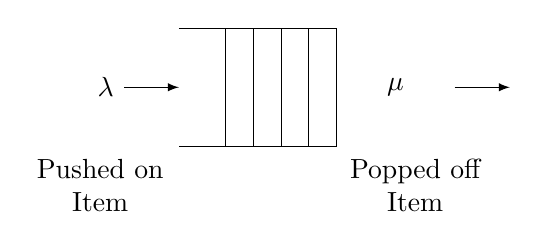
\begin{tikzpicture}[>=latex]
        % the rectangle with vertical rules
        \draw (0,0) -- ++(2cm,0) -- ++(0,-1.5cm) -- ++(-2cm,0);
        \foreach \i in {1,...,4}
          \draw (2cm-\i*10pt,0) -- +(0,-1.5cm);
        
        % % the circle
        % \draw (2.75,-0.75cm) circle [radius=0.75cm];
        
        % the arrows and labels
        \draw[->] (3.5,-0.75) -- +(20pt,0);
        \draw[<-] (0,-0.75) -- +(-20pt,0) node[left] {$\lambda$};
        \node at (2.75,-0.75cm) {$\mu$};
        \node[align=center] at (-1cm,-2cm) {Pushed on \\ Item};
        \node[align=center] at (3cm,-2cm) {Popped off\\ Item};
        \end{tikzpicture}
\end{frame}
\begin{frame}[fragile]
\frametitle{Code for BFS}
     \begin{lstlisting}[language=Python]
     graph = []
     queue = [] 
     seen = [] 
     queue.push(0) #add start node to the front
     while(not queue.isempty()):
        current = queue.pop()
        for adj in graph[current]: 
            if adj not in seen:
                queue.push(adj)
  \end{lstlisting}
\end{frame}
\begin{frame}[fragile]
\frametitle{More competitive code}
    \begin{lstlisting}[language=Python]
    struct node {
        int val;
        vector<node*> edges;
    };
    void bfs(node *root){
        queue<node*> q;
        q.push(root);
        node *curr;
        while(q.size() > 0){
            curr = q.front();
            q.pop();
            cout << curr->val << " ";
            for(node *edge : curr->edges){
                q.push(edge);
            }
        }
 \end{lstlisting}
    
\end{frame}
\begin{frame}{Depth First Search}
\centering
\begin{tikzpicture}[scale=2.5, auto,swap]
    % First we draw the vertices
    \foreach \pos/\name in {
                                {(1.5,2.5)/0},
                                {(0.25,1.75)/1}, {(2.75,1.75)/2},
                                {(-0.25,1)/3}, {(0.75,1)/4}, {(2.25,1)/5}, {(3.25,1)/6},
                                {(-0.25,0.25)/7}, {(0.5,0.25)/8}, {(1,0.25)/9}, {(1.75,0.25)/10}, {(2.25,0.25)/11}, {(2.75,0.25)/12}}
        \node[vertex] (\name) at \pos {$\name$};
    % Connect vertices with edges and draw weights
    \foreach \source/ \dest /\weight in {0/1/, 0/2/,1/3/,1/4/,
                                         3/7/, 4/8/,4/9/,
                                         0/2/,2/5/,
                                         2/6/,5/10/,5/11/,5/12/}
        \path[edge] (\source) -- node[weight] {$\weight$} (\dest);
    % Start animating the vertex and edge selection. 
    \foreach \vertex / \fr in {0/1,1/2,2/2,3/3,7/4,4/3, 8/5,9/5, 5/8,6/8, 10/9,11/9,12/9}
        \path<\fr-> node[selected vertex] at (\vertex) {$\vertex$};
    % For convenience we use a background layer to highlight edges
    % This way we don't have to worry about the highlighting covering
    % weight labels. 
    \begin{pgfonlayer}{background}
        \pause
        \foreach \source / \dest in {0/1,1/3,3/7,1/4,4/8,4/9, 0/2,2/5,5/10,5/11,5/12,2/6}
            \path<+->[selected edge] (\source.center) -- (\dest.center);
        % \foreach \source / \dest / \fr in {d/b/4,d/e/5,e/f/5,b/c/6,f/g/7}
        %     \path<\fr->[ignored edge] (\source.center) -- (\dest.center);
    \end{pgfonlayer}
\end{tikzpicture}
    
\end{frame}
\begin{frame}{DFS}
\centering
\begin{tikzpicture}[scale=2.5, auto,swap]
    % First we draw the vertices
    \foreach \pos/\name in {
                                {(1.5,2.5)/0},
                                {(0.25,1.75)/1}, {(2.75,1.75)/2},
                                {(-0.25,1)/3}, {(0.75,1)/4}, {(2.25,1)/5}, {(3.25,1)/6},
                                {(-0.25,0.25)/7}, {(0.5,0.25)/8}, {(1,0.25)/9}, {(1.75,0.25)/10}, {(2.25,0.25)/11}, {(2.75,0.25)/12}}
        \node[vertex] (\name) at \pos {$\name$};
    % Connect vertices with edges and draw weights
    \foreach \source/ \dest /\weight in {0/1/, 0/2/,1/3/,1/4/,
                                         3/7/, 4/8/,4/9/,
                                         0/2/,2/5/,
                                         2/6/,5/10/,5/11/,5/12/}
        \path[edge] (\source) -- node[weight] {$\weight$} (\dest);;
  \draw[->,blue,rounded corners,dashed,line width=0.7pt,scale=0.5]
    ($(0) + (-0.4,0.2)$) --
    ($(1) +(-0.3,0.4)$) --
    ($(1) +(-0.6,0.0)$) --
    ($(3)  +(-0.4,0.3)$) --
    ($(3)  +(-0.5,0.0)$) --
    ($(7)  +(-0.5,0.0)$) --
    ($(7)  +(-0.4,-0.35)$) --
    ($(7)  +(0.0,-0.5)$) --
    ($(7)  +(0.4,-0.35)$) --
    ($(7)  +(0.5,0.0)$) --
%    ($(3)  +(0.45,-0.2)$) --
    ($(3)  +(0.45,0.0)$) --
    ($(1)  +(0.0,-0.4)$) --
    ($(4)  +(-0.45,0.0)$) --
    ($(8)  +(-0.45,0.0)$) --
    ($(8)  +(-0.35,-0.35)$) --
    ($(8)  +(0.0,-0.45)$) --
    ($(8)  +(0.35,-0.35)$) --
    ($(8)  +(0.4,0.0)$) --
    ($(4)  +(0.0,-0.4)$) --
    ($(9)  +(-0.45,0.0)$) --
    ($(9)  +(-0.35,-0.35)$) --
    ($(9)  +(0.0,-0.45)$) --
    ($(9)  +(0.35,-0.35)$) --
    ($(9)  +(0.45,0.0)$) --
    ($(4)  +(0.4,0.2)$) --
    ($(1)  +(0.4,0.0)$) --
    ($(0)  +(0.0,-0.4)$) --
    ($(2)  +(-0.4,0.0)$) --
%    ($(5)  +(-0.6,0.0)$) --
    ($(10)  +(-0.5,0.1)$) --
    ($(10)  +(-0.4,-0.35)$) --
    ($(10)  +(0.0,-0.5)$) --
    ($(10)  +(0.4,-0.3)$) --
    ($(5)  +(-0.15,-0.4)$) --
    ($(11)  +(-0.5,0.0)$) --
    ($(11)  +(-0.4,-0.35)$) --
    ($(11)  +(0.0,-0.5)$) --
    ($(11)  +(0.4,-0.35)$) --
    ($(11)  +(0.5,0.0)$) --
    ($(5)  +(0.15,-0.4)$) --
    ($(12)  +(-0.5,0.0)$) --
    ($(12)  +(-0.4,-0.35)$) --
    ($(12)  +(0.0,-0.5)$) --
    ($(12)  +(0.4,-0.35)$) --
    ($(12)  +(0.5,0.2)$) --
    ($(5)  +(0.4,0.0)$) --
    ($(2)  +(0.0,-0.4)$) --
    ($(6)  +(-0.5,0.0)$) --
    ($(6)  +(-0.4,-0.35)$) --
    ($(6)  +(0.0,-0.5)$) --
    ($(6)  +(0.4,-0.35)$) --
    ($(6)  +(0.5,0.1)$) --
    ($(2) +(0.6,0.0)$) --
    ($(2) +(0.3,0.4)$) --
    ($(0) + (0.4,0.2)$);
\end{tikzpicture}
\end{frame}
\begin{frame}{How to implement}
    \begin{itemize}
        \item see what nodes are adjacent to us
        \item chose one and go down it
        \item look at what nodes are adjacent to that one
        \item explore one of them 
        \item repeat until there are no nodes left to explore down one node. go to the next.
    \end{itemize}
\end{frame}
\begin{frame}{Stacks}
    \begin{columns}
        \column{0.5\textwidth}
            \begin{itemize}
                \item first in - first out
                \item items are pushed onto the stack and popped right back off the top
            \end{itemize}
        \column{0.4\textwidth}
        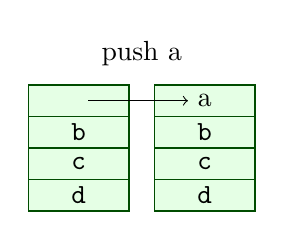
\begin{tikzpicture}[scale=0.4]
        \draw (2, 0.5) node (Otm) {
    \begin{tabular}{c}
      push a
    \end{tabular}
  };

  \drawstruct{(0,0)}
  \structcell[freecell]{~} \coordinate (Atm) at (currentcell.east);
  \structcell[freecell]{\texttt{b}}
  \structcell[freecell]{\texttt{c}}
    \structcell[freecell]{\texttt{d}}

  \drawstruct{(4,0)}
  \structcell[freecell]{a} \coordinate (Btm) at (currentcell.west);
  \structcell[freecell]{\texttt{b}}
  \structcell[freecell]{\texttt{c}}
  \structcell[freecell]{\texttt{d}}
 

  \draw[->] (Atm) -- (Btm);
\end{tikzpicture}

    \end{columns}
\end{frame}
\begin{frame}[fragile]
\frametitle{Code for DFS}
     \begin{lstlisting}[language=Python]
     graph = []
     queue = [] 
     seen = [] 
     stack.push(0) #the only difference
     while(not queue.isempty()):
        current = queue.pop()
        for adj in graph[current]: 
            if adj not in seen:
                queue.push(adj)
  \end{lstlisting}
\end{frame}
\begin{frame}{Shortest Paths}
    \begin{itemize}
        \item How do I get from point A to point B as quickly as possible?
        \item How can I be sure that a path from A to B is better than all other possible ones?
    \end{itemize}
\end{frame}
\begin{frame}{Priority first search}
    \begin{itemize}
        \item As soon as we see a node just it into a queue
        \item order this queue by some means so the node we want the most is at the start
        \item greedily select the highest priority node
    \end{itemize}
\end{frame}
\begin{frame}{different versions of Priority}
    \begin{itemize}
        \item in BFS priority is node we discovered first
        \item in DFS priority is node we have most recently seen
        \item in Dijkstra's shortest path priority is \textbf{the node which is closest to us}
    \end{itemize}
\end{frame}
\begin{frame}{Dijkstra's Algorithm}
    \begin{itemize}
        \item start at some node and look at adjacent ones
        \item choose the one with the lowest weight and explore it
        \item for all paths coming off this new node keep in mind the distance will be that nodes wight plus the one that came before
        \item continue to greedily select nodes until all nodes have been seen
    \end{itemize}
\end{frame}
\begin{frame}{how to implement Dijkstra's?}
    The key will be a priority queue, the rest is the same as before
\end{frame}
\begin{frame}[fragile]
    \frametitle{Code for Dijkstra's}
             \begin{lstlisting}[language=Python]
def dijkstra(adj, src):
    pq = []
    rv = [sys.maxsize for _ in range(len(adj))]
    rv[src] = 0
    heapq.heappush(pq,(0, src))
    while(len(pq) > 0):
    	_, u = heapq.heappop(pq)
    	for v, w in adj[u]:
    		if(rv[v] > rv[u] + w):
    		rv[v] = rv[u] + w
    		heapq.heappush(pq, (-rv[v], v))
    return rv
  \end{lstlisting}
    \end{frame}
\begin{frame}[fragile]
    \frametitle{More competitive implementation}
    \begin{lstlisting}[language=c,basicstyle=\small]
typedef pair<int, int> pii;

vector<int> dijkstra(vector<list<pii>>adj, int src){
    priority_queue<pii, vector<pii>, greater<pii>> pq;
    vector<int> rv(adj.size(), INT_MAX);
    rv[src] = 0;
    pq.push({0, src});
    int u, v, w;
    while(pq.size() > 0){
    	u = pq.top().second;
    	pq.pop();
    	for(auto i = adj[u].begin(); i != adj[u].end(); i++){
    		v = (*i).first;
    		w = (*i).second;
    		if(rv[v] > rv[u] + w){
    			rv[v] = rv[u] + w;
    			pq.push({rv[v], v});
		}
	}
}
return rv;
}
    \end{lstlisting}
\end{frame}
\begin{frame}{Mimimum spanning tree}
    Simply the least number of edges you have to add to connect every node in a graph
    \vspace{0.5cm}
    \begin{columns}
        \column{0.4\textwidth}
             \tikzset{vertex/.style={draw=red!40!white, black=red, fill=red!10!white, shape=circle, inner sep=0.5pt, minimum size=16pt}}
        \begin{tikzpicture}[
            g1v/.style={vertex,draw=red!40!white, black=red, fill=white!10!white},
            g2v/.style={vertex,draw=blue!40!white, black=blue, fill=white!10!white},
            g3v/.style={vertex,draw=green!40!white, black=green, fill=white!10!white},
            g4v/.style={vertex,draw=green!40!white, black=green, fill=red!10!white},
            scale=1
        ]
        \node[g1v] (0) at (0,0.75) {0};

        \node[g1v] (1) at (1.5,1.5) {1};
        \node[g1v] (2) at (1.5,0) {2};

        \node[g2v] (3) at (3,1.5) {3};
        \node[g3v] (4) at (3,0) {4};

        \node[g1v] (5) at (4.5,1.5) {5};

        \draw[] (0) --  (1);
        \draw[] (1) --  (2);
        \draw[] (1) -- (3);
        \draw[] (1) -- (4);
        \draw[] (2) -- (0);
        \draw[] (2) -- (4);
        \draw[thick] (3) -- (5);
    \end{tikzpicture}
    \column{0.5\textwidth}
        \begin{tikzpicture}[
            g1v/.style={vertex,draw=red!40!white, black=red, fill=white!10!white},
            g2v/.style={vertex,draw=blue!40!white, black=blue, fill=white!10!white},
            g3v/.style={vertex,draw=green!40!white, black=green, fill=white!10!white},
            g4v/.style={vertex,draw=green!40!white, black=green, fill=red!10!white},
            scale=1
        ]
        \node[g1v] (0) at (0,0.75) {0};

        \node[g1v] (1) at (1.5,1.5) {1};
        \node[g1v] (2) at (1.5,0) {2};

        \node[g2v] (3) at (3,1.5) {3};
        \node[g3v] (4) at (3,0) {4};

        \node[g1v] (5) at (4.5,1.5) {5};

        \draw[] (0) --  (1);
        \draw[] (1) --  (2);
        \draw[] (1) -- (3);
        \draw[] (1) -- (4);
        \draw[] (2) -- (0);
        \draw[thick] (3) -- (5);
    \end{tikzpicture}
    \end{columns}
\end{frame}
\begin{frame}{Prim's algorithm}
    \begin{itemize}
        \item very much like Dijkstra's in that start at a node
        \item look at adjacent nodes add to priority queue
        \item greedily select lowest weight one
        \item repeat till all nodes have been seen
    \end{itemize}
\end{frame}
\begin{frame}
\frametitle{Prim's algorithm}

%% Adjacency matrix of graph
%% \  a  b  c  d  e  f  g
%% a  x  7     5
%% b  7  x  8  9  7
%% c     8  x     5
%% d  5  9     x 15  6
%% e     7  5 15  x  8  9
%% f           6  8  x 11
%% g              9  11 x

\tikzstyle{vertex}=[circle,draw=blue!40!white, black=blue, fill=white!10!white]
\tikzstyle{selected vertex} = [vertex, fill=red!24]
\tikzstyle{edge} = [draw,thick,-]
\tikzstyle{weight} = [font=\small]
\tikzstyle{selected edge} = [draw,line width=5pt,-,red!50]
\tikzstyle{ignored edge} = [draw,line width=5pt,-,black!20]

\begin{figure}
\begin{tikzpicture}[scale=1.8, auto,swap]
    % Draw a 7,11 network
    % First we draw the vertices
    \foreach \pos/\name in {{(0,2)/a}, {(2,1)/b}, {(4,1)/c},
                            {(0,0)/d}, {(3,0)/e}, {(2,-1)/f}, {(4,-1)/g}}
        \node[vertex] (\name) at \pos {$\name$};
    % Connect vertices with edges and draw weights
    \foreach \source/ \dest /\weight in {b/a/7, c/b/8,d/a/5,d/b/9,
                                         e/b/7, e/c/5,e/d/15,
                                         f/d/6,f/e/8,
                                         g/e/9,g/f/11}
        \path[edge] (\source) -- node[weight] {$\weight$} (\dest);
    % Start animating the vertex and edge selection. 
    \foreach \vertex / \fr in {d/1,a/2,f/3,b/4,e/5,c/6,g/7}
        \path<\fr-> node[selected vertex] at (\vertex) {$\vertex$};
    % For convenience we use a background layer to highlight edges
    % This way we don't have to worry about the highlighting covering
    % weight labels. 
    \begin{pgfonlayer}{background}
        \pause
        \foreach \source / \dest in {d/a,d/f,a/b,b/e,e/c,e/g}
            \path<+->[selected edge] (\source.center) -- (\dest.center);
        \foreach \source / \dest / \fr in {d/b/4,d/e/5,e/f/5,b/c/6,f/g/7}
            \path<\fr->[ignored edge] (\source.center) -- (\dest.center);
    \end{pgfonlayer}
\end{tikzpicture}
\end{figure}

\end{frame}

\end{document}

